% Im header stehen die Grundeinstellungen des Dokuments
\documentclass[12pt,a4paper]{article} % 12 Punkte Schrift, A4 Papier
\usepackage[utf8]{inputenc} 
\usepackage[ngerman]{babel} % Passt alle automatischen Texte an. 
%\usepackage[english]{babel} % Diese Variante verwenden, fall man eine Arbeit auf Englisch schreibt.

\parindent=0cm
\parskip=0.3cm
\linespread{1.5}




% Ein paar standard Pakete. Man muss genau wissen, wofür alle gebraucht werden...
\usepackage{amsmath}
\usepackage{amsfonts}
\usepackage{amssymb}
\usepackage{pdfpages}
\usepackage{hyperref}
\usepackage{csquotes}
\usepackage{graphicx}

\graphicspath{{images/}}


% für Schachbretter
% \usepackage{xskak,chessboard}

\usepackage[
    backend=biber,
    style=apa,
    sortlocale=de_DE,
    natbib=true,
    url=false,
    doi=false,
    sortcites=true,
    sorting=nyt,
    isbn=false,
    hyperref=true,
    backref=false,
    giveninits=false,
    eprint=false]{biblatex}
\addbibresource{references/bibliography.bib}

% Informationen für die Titelseite
\title{Beispiel für eine Maturarbeit}
\date{\today}
\author{Susy Muster}




% Der Anfang des Dokuments
\begin{document}



\maketitle % Hier wird die Titelseite mit den obigen Informationen eingefügt. Falls man eine "kunstvollere" Titelseite mit einem anderen Programm erstellen möchte, kann man sie hier einfügen. Dafür muss man die Titelseite im gleichen Verzeichnis (z.B. mit dem Namen TitelseiteMA2016.pdf) im pdf Format ablegen und mit dem Befehl
% \includepdf{TitelseiteMA2016}
% wird sie dann eingefügt.











\newpage % Eine neue Seite wird begonnen...
\tableofcontents % Hier wird automatisch das Inhaltsverzeichnis eingefügt. Achtung: Änderungen werden erst nach dem zweiten kompilieren sichtbar.











\newpage

\section{Struktur}

Ein Abschnitt wird mit diesem Befehl kreiert:
\begin{verbatim}
\section{Einleitung}
\end{verbatim}

Das sieht dann so aus:

% Die Grundstruktur einer Arbeit:
\section{Einleitung}
Hier kommt text\ldots 

Unterabschnitte werden so dargestellt:

\begin{verbatim}
\subsection{Quellen und Zitate}
\end{verbatim}

und sehen dann so aus:

\subsection{Quellen und Zitate}

% Mit einer Leerzeile wird ein neuer Abschnitt begonnen


Wenn man auf eine Quelle verweisen möchte, verwendet man den \verb|\citet{}| oder \verb|\citep{}| Befehl \citep{example}. Man kann dann auch eine zweite Quelle zitieren: ``Life finds a way" \citep{buch2}.

\citet{example} sagt \dots


\newpage




\section{Bilder}

Bilder/Graphiken werden mit dem folgenden Befehl eingefügt:

\begin{verbatim}
\begin{figure}[h]
\centering 
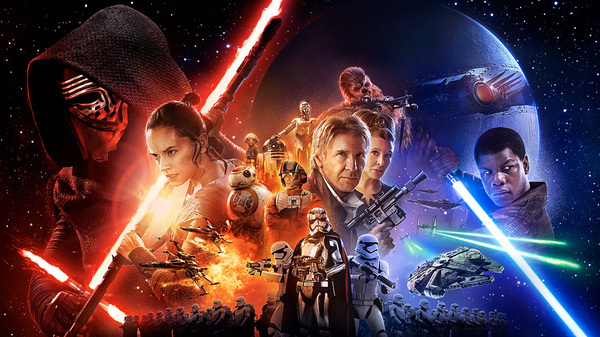
\includegraphics[width=0.5\textwidth]{star_wars.jpeg}
\caption{Ein erstes Bild \cite{sw16}}
\end{figure}
\end{verbatim}

Die \verb|figure| Umgebung zeichnet ein Bild, das \verb|[h]| heisst, dass die Graphik möglichst direkt hier im Text eingebettet werden soll.

Das sieht dann so aus:

\begin{figure}[h] % Die "figure" Umgebung 
\centering % Damit wird das Bild zentriert
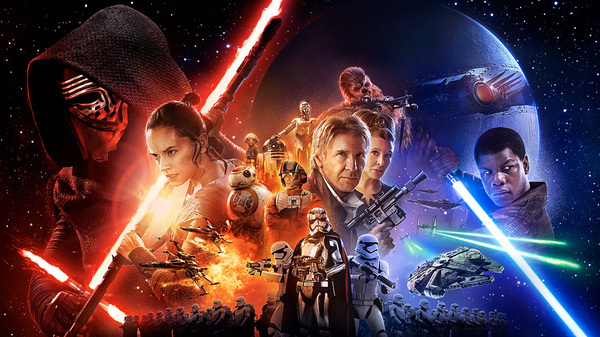
\includegraphics[width=0.5\textwidth]{star_wars.jpeg} % Hier wird ein Bild eingefügt, das im selben Verzeichnis abgelegt wurde. Es wird so vergrössert/verkleinert, dass es auf die halbe Textbreite passt.
\caption{Ein erstes Bild \citep{star-wars}}
\end{figure}

Bilder tauchen automatisch im Bildverzeichnis auf.


\newpage

% \section{Schachbretter}
% Schachbretter mit bestimmten Positionen, können in der FEN Notation angegeben werden (Die Forsyth-Edwards-Notation (FEN) oder in der erweiterten Form (X-FEN) ist eine Kurznotation, mit der jede beliebige Brettstellung im Schach niedergeschrieben werden kann.\cite{fen-wiki}):

% \begin{verbatim}
% \begin{figure}[h]
% \centering
% \chessboard[setfen=1n1Rkb1r/p4ppp/4q3/4p1B1/4P3/8/PPP2PPP/2K5 b k - 1 17]
% \caption{Schachmatt! (Morphy vs. Karl von Braunschweig und Graf Isoard, 1858)}
% \end{figure}
% \end{verbatim}

% Das sieht dann so aus:
% \setchessboard{showmover=false}


% \begin{figure}[h]
% \centering
% \chessboard[setfen=1n1Rkb1r/p4ppp/4q3/4p1B1/4P3/8/PPP2PPP/2K5 b k - 1 17]
% \caption{Schachmatt! (Morphy vs. Karl von Braunschweig und Graf Isoard, 1858)}
% \end{figure}

% \newpage

% Züge können mit dem Befehl \verb|markmoves| eingezeichnet werden:

% \begin{verbatim}
% \begin{figure}[h]
% \centering
% \chessboard[smallboard,
% setpieces={Ra1,Rh1,Ke1,ke8,rh8,ra8,Ne6,bb4},
% arrow=to,linewidth=0.2ex,
% pgfstyle=knightmove,
% shortenstart=0.4em,
% color=red!80,
% markmoves={e6-d8,e6-f8},
% pgfstyle=straightmove,
% shortenstart=0.4em,
% color=red!80,
% markmoves={b4-e1},
% ]
% \caption{Keine Rochaden sind möglich}
% \end{figure}
% \end{verbatim}

% \begin{figure}[h]
% \centering
% \chessboard[smallboard,
% setpieces={Ra1,Rh1,Ke1,ke8,rh8,ra8,Ne6,bb4},
% arrow=to,linewidth=0.2ex,
% pgfstyle=knightmove,
% shortenstart=0.4em,
% color=red!80,
% markmoves={e6-d8,e6-f8},
% pgfstyle=straightmove,
% shortenstart=0.4em,
% color=red!80,
% markmoves={b4-e1},
% ]
% \caption{Keine Rochaden sind möglich}
% \end{figure}

% \newpage



\section{Schlussfolgerungen}
\newpage




% Hier beginnt der Anhang
\appendix
\section{Anhang}
\newpage





\section{Bilderverzeichnis}
\listoffigures



\newpage

\printbibliography







































\end{document}